\documentclass[11pt]{article}   
\usepackage{fullpage}
\usepackage{amsfonts}
\usepackage{amssymb}
\usepackage{amsmath}
\usepackage{xcolor}
\usepackage{graphicx}

\newcommand{\F}{\mathbb{F}}
\newcommand{\np}{\mathop{\rm NP}}
%\newcommand{\binom}[2]{{#1 \choose #2}}
\newcommand{\Z}{{\mathbb Z}}
\newcommand{\vol}{\mathop{\rm Vol}}
\newcommand{\conp}{\mathop{\rm co-NP}}
\newcommand{\atisp}{\mathop{\rm ATISP}}
\renewcommand{\vec}[1]{{\mathbf #1}}
\newcommand{\cupdot}{\mathbin{\mathaccent\cdot\cup}}
\newcommand{\mmod}[1]{\ (\mathrm{mod}\ #1)}  

\setlength{\parskip}{\medskipamount}
\setlength{\parindent}{0in}
%\input{dansmacs}


\begin{document}
	
	\section*{CS 121 Homework 3: Fall
		2020}\label{cs-121-homework-zero-fall-2020}
	
	\textbf{Some policies:} (See the course policy at  {\tt http://madhu.seas.harvard.edu/courses/Fall2020/policy.html} for the
	full policies.)
	
	\begin{itemize}
		\item
		{\bf Collaboration:} You can collaborate with other students that are currently enrolled in
		this course (or, in the case of homework zero, planning to enroll in
		this course) in brainstorming and thinking through approaches to
		solutions but you should write the solutions on your own and cannot
		share them with other students. 
		\item
		{\bf Owning your solution:} Always make sure that you ``own'' your solutions to this other problem
		sets. That is, you should always first grapple with the problems on
		your own, and even if you participate in brainstorming sessions, make
		sure that you completely understand the ideas and details underlying
		the solution. This is in your interest as it ensures you have a solid
		understanding of the course material, and will help in the midterms
		and final. Getting 80\% of the problem
		set questions right on your own will be much better to both your
		understanding than getting 100\% of the questions through
		gathering hints from others without true understanding.
		\item
		{\bf Serious violations:} Sharing questions or solutions with anyone outside this course,
		including posting on outside websites, is a violation of the honor
		code policy. Collaborating with anyone except students currently
		taking this course or using material from past years from this or
		other courses is a violation of the honor code policy.
		\item
		{\bf Submission Format:} The submitted PDF should be typed and in the same format and
		pagination as ours. Please include the text of the problems and write
		\textbf{Solution X:} before your solution. Please mark in gradescope 
		the pages where
		the solution to each question appears. Points will be deducted if you
		submit in a different format.
		\item {\bf Late Day Policy:} To give students some flexibility to manage your schedule, you are allowed a net total of {\bf eight} late days through the semester, but you may not take more than {\bf two} late days on any single problem set. No exceptions to this policy. 
	\end{itemize}
	
	\textbf{By writing my name here I affirm that I am aware of all policies
		and abided by them while working on this problem set:}
	
	\textbf{Your name:} Todd Morrill
	
	\textbf{Collaborators:} (List here names of anyone you discussed
	problems or ideas for solutions with)
	
	% For homeworks 1 through n
	\textbf{No. of late days used on previous psets (not including Homework Zero): }0\\
	\textbf{No. of late days used after including this pset: } 1
	
	
	\newpage
	
	\subsection*{Questions}\label{questions}
	
Please solve the following problems. Some of these might be harder than
the others, so don't despair if they require more time to think or you
can't do them all. Just do your best. Also, you should only attempt the
bonus questions if you have the time to do so. If you don't have a proof
for a certain statement, be upfront about it. You can always explain
clearly what you are able to prove and the point at which you were
stuck. 
%Also, for a non bonus question, 
You can always simply write
\textbf{``I don't know''} and you will get 15 percent of the credit for
this problem. If you are stuck on this problem set, you can use Piazza to
send a private message to all staff.

\iffalse{ \textbf{Note on ``bonus'' questions:} There is no difference between
``bonus'' points and regular points. The indication ``bonus'' is just a
helpful hint for you: it means that the question might be harder, and
you might not want to spend inordinate amounts of time on it. Also, the
total point value of all non bonus questions will always be at least
100, so you can get a perfect grade on the problem set component of this
course without ever solving a bonus question.

\textbf{Note on reading the textbook:} If you are stuck on some of the
problems, try consulting the book to 1) understand the concepts the
question is referencing, and 2) review the way similar theorems are
proved in the book. Some helpful sections of the book for this problem
set are: Chapter 8 (for Rice's Theorem), Chapter 10 (to see solved
reductions to \(HALT\) and \(HALTONZERO\)), and Chapter 9 (for proofs
utilizing the pumping lemma and other useful proofs regarding the
computability/halting of regular expressions).

}\fi 

\newcommand{\N}{\mathbb{N}} 
\newcommand{\XOR}{\mathrm{XOR}} 
\newcommand{\Size}{\mathrm{SIZE}} 

\newpage

\textbf{Problem 1:}
Recall that in section, we defined the function $LOOKUP_k: \{0,1\}^{2^k + k} \to \{0,1\}$ by 
$$LOOKUP_k(X[0], X[1], \ldots, X[2^{k}-1], i[0], \ldots, i[k-1]) = X[i[0] + 2 i[1] + \cdots + 2^{k-1}i[k-1]]$$ 
and proved that there exists a circuit with $O(2^k)$ gates that computes $LOOKUP_k$. We'll write $LOOKUP_k(X, i)$ as shorthand for $LOOKUP_k(X[0], X[1], \ldots, X[2^{k}-1], i[0], \ldots, i[k-1])$.

\textbf{Problem 1.1 (8 points)} Prove that $LOOKUP_k(X,i)$ cannot be computed by circuits $C$ of size $o(2^k)$.

\textbf{Solution 1.1:}% (write your solution here)

The proof is by contradiction. Suppose there is a circuit $C$ of size $o(2^k)$ that computes $LOOKUP_k(X,i)$. If this were the case, $LOOKUP_k(X,i)$ would ignore at least one of the input bits since the input size is $2^k + k$. This can be broken down into two cases.

The first case is when one of the $2^k$ return values is ignored, in which case toggling this ignored value from 0 to 1 would not change the value returned by $LOOKUP_k(X,i)$.

The second case is when one of the $k$ bits in index $i$ is ignored. If this were the case then toggling that ignored bit from 0 to 1 would again not change the value returned by $LOOKUP_k(X,i)$.

In both cases, toggling the ignored bit changes the function but does not change the circuit. Therefore, we have found a contradiction and cannot compute $LOOKUP_k(X,i)$ with a circuit $C$ of size $o(2^k)$.

\textbf{Problem 1.2 (4 points)} Prove that for every $X \in \{0,1\}^{2^k}$ there exists a circuit $C(X)$\footnote{That is, the circuit may depend on $X$.} of size $o(2^k)$ that computes $LOOKUP_k(X,i)$. (You may use results stated but not proved in lecture.)

\textbf{Solution 1.2:}% (write your solution here)

We can hardcode a particular $X \in \{0,1\}^{2^k}$ into the circuit C(X). In this case, we only need $k$ bits of input for the circuit, which act as an index into the hardcoded values. By Theorem 4.15 from the textbook, there exists a constant $c > 0$ such that for every $k > 0$ and function $f: \{0, 1\}^k \to \{0, 1\}$, there is a NAND-CIRC program with at most $c2^k / k$ lines that computes the function f. Since $c2^k / k = o(2^k)$ there exists a circuit C(X) of size $o(2^k)$ that computes $LOOKUP_k(X,i)$ for every $X \in \{0,1\}^{2^k}$, which completes the proof.

\textbf{Problem 1.3 (8 points)} Prove that there exists $X \in \{0,1\}^{2^k}$ such that there does not exist a circuit $C(X)$\footnotemark[1] of size $o(2^{\sqrt k})$ that computes $LOOKUP_k(X,i)$.

\textbf{Solution 1.3:}% (write your solution here)

We can hardcode a particular $X \in \{0,1\}^{2^k}$ into the circuit C(X). In this case, we only need $k$ bits of input for the circuit, which act as an index into the hardcoded values. By Theorem 5.3 from the textbook, there is a constant
$\delta > 0$, such that for every sufficiently large $k$, there is a function
$f: \{0, 1\}^k \to \{0, 1\}$ such that $f \notin SIZE(\delta \cdot 2^k / k)$. That is, the shortest NAND-CIRC program to compute $f$ requires more than $\delta \cdot 2^k / k $ lines. Since $\delta \cdot 2^k / k \neq o(2^{\sqrt k})$, there exists $X \in \{0,1\}^{2^k}$ such that there does not exist a circuit $C(X)$ of size $o(2^{\sqrt k})$ that computes $LOOKUP_k(X,i)$, which completes the proof.

\newpage

\newcommand{\BSize}{\mathrm{BSIZE}}

\textbf{Problem 2:}
Recall that 
$$\Size_{n,m}(s) = \{f:\{0,1\}^n \to \{0,1\}^m | \exists \mbox{ NAND circuit $C$ of at most $s$ gates s.t. $C$ computes $f$ }\}.$$ 
Let $\BSize(s) = \cup_{n \in \N}  \Size_{n,1}(s)$ represent the set of Boolean functions (i.e., those whose output is in $\{0,1\}$) that are computable by NAND circuits of size at most $s$.

Prove the following:

\textbf{Problem 2.1 (3 points):} $|\BSize(s)| =  2^{O(s \log s)}$. 

\textbf{Solution 2.1:}% (write your solution here)

Theorem 5.2 from the textbook states that for every $s \in \N$, $|\Size(s)| =  2^{O(s \log s)}$. That is, there are at most $2^{O(s \log s)}$ functions computed by NAND-CIRC programs of at most $s$ lines. Since $\BSize(s)$ is a subset of $\Size(s)$ by definition, we can conclude that $|\BSize(s)| =  2^{O(s \log s)}$.


\textbf{Problem 2.2 (15 points):} $|\BSize(s)| = 2^{\Omega(s)}$.

\textbf{Solution 2.2:}% (write your solution here)

We know by theorem 4.15 from the textbook that there exists a NAND-CIRC program with at most $c \cdot 2^n / n$ lines that computes the function $f$. This means that if $(2^n / n) < s$, then we can sum the number of functions $f_n: \{0, 1\}^n \to \{0, 1\}$ for all values of $n$ satisfying this condition, where the size of these sets is $2^{2^n}$.

\begin{equation} \label{eq1}
\begin{split}
	|\BSize(s)| & = \sum_{n s.t. (2^n/n) < s}{2^{2^n}} \\
	& > \sum_{n s.t. (2^n) < s}{2^{2^n}} = \sum_{n=1}^{\lfloor \log_2{s} \rfloor}{2^{2^n}} \\ 
	& > 2^{2^{\lfloor \log_2{s} \rfloor}} \approxeq 2^{2^{\log_2{s}}} \\
	& = 2^{s}\\
\end{split}
\end{equation}

This implies that $|\BSize(s)| = 2^{\Omega(s)}$, which is what we wanted to show.

\textbf{Problem 2.3 (2 points):} $\BSize(s) \subsetneq \BSize(s^2)$, for every sufficiently large $s$.  

\textbf{Solution 2.3:}% (write your solution here)

We know that by \textbf{Solution 2.1}, $|\BSize(s)| =  2^{O(s \log s)}$ and that by \textbf{Solution 2.2}
$|\BSize(s^2)| = 2^{\Omega(s^2)}$. These two facts imply that the cardinality of these two sets are distinct and therefore $\BSize(s) \subsetneq \BSize(s^2)$ for every sufficiently large $s$.

\iffalse{  % Version 2 - revised to fix problem with size definition
\textbf{Problem 2:}
Recall that 
$$\Size_{n,m}(s) = \{f:\{0,1\}^n \to \{0,1\}^m | \exists \mbox{ NAND circuit $C$ of at most $s$ gates s.t. $C$ computes $f$ }\}.$$ 
Let $\Size(s) = \cup_{n \in \N} \cup_{m \in \N} \Size_{n,m}(s)$. 
Prove the following:

\textbf{Problem 2.1 (6 points):} $|\Size(s)| =  2^{O(s \log s)}$. 

\textbf{Solution 2.1:}% (write your solution here)

\textbf{Problem 2.2 (12 points):} $|\Size(s)| = 2^{\Omega(s)}$.

\textbf{Solution 2.2:}% (write your solution here)

\textbf{Problem 2.3 (2 points):} $\Size(s) \subsetneq \Size(s^2)$, for every sufficiently large $s$.  

\textbf{Solution 2.3:}% (write your solution here)
}\fi 


\iffalse % Version 1 - Removed because they were covered in 121.5:
\textbf{Problem 2.2 (20 points):}
Let $f,g:\{0,1\}^n \to \{0,1\}$ be two functions that differ one only one input. I.e., there exists $a \in \{0,1\}^n$ such that $f(a) \ne g(a)$ and $f(b) = g(b)$ for all $b \in \{0,1\}^n \setminus \{a\}$. Let $S(f)$ denote the size of the smallest NAND circuit computing $f$ and let $S(g)$ denote the size of the smallest circuit computing $S(g)$. (1) Prove that $S(f) \leq S(g) + 10 n$. 

\textbf{Solution 2.2:} (write your solution here)

\textbf{Problem 2.3 (Bonus, Optional, 0 points):}
Use Problem 2.2 to prove that if $n \leq s \leq 2^n/n - 10n$ then $\Size_{n,1}(s) \subsetneq \Size_{n,1}(s+10n)$. 

\textbf{Solution 2.3:} (write your solution here)
\fi

%{\color{red} In questions below, make sure notation/terminology is consistent with what we use in class. Current notation supposedly based on Barak's book. }

\newpage 

\textbf{Problem 3.1 (15 points):} Describe the set of inputs accepted by the following DFA with 4 states given by $(T,S)$ where $S = \{1,3\}$ and $T$ is given by the following table:
\[
\begin{array}{||c||c|c|c|c||}
\hline
\hline
\mathrm{Input}~\downarrow ~\backslash~ \mathrm{State}~\to & 0 & 1 & 2 & 3 \\
\hline
\hline
0 & 0 & 0 & 1 & 1 \\
\hline
1 & 2 & 2 & 3 & 3 \\
\hline
\hline
\end{array}
\]

\textbf{Solution 3.1:}% (write your solution here)

The set of inputs accepted by this DFA can be represented by its equivalent regular expression: $(0|1)^*1(0|1)$. In words, this DFA (and equivalent regex) accept strings where the second to last bit of the string is 1. This is correct because the DFA remains in state transitions to state 0 are always on a 0 input, transitions to state 1 (an accept state) are always \textit{after} a 1 input, transitions to state 2 are always on a 0 input, and transitions to state 3 (an accept state) are always \textit{after} a 1 input.
 
\textbf{Problem 3.2 (bonus, 0 points):} For all $n$, find, with proof, a regular expression with $10n + 100$ characters that's equivalent to some DFA with $2^n$ states and not equivalent to any DFA with $2^n - 1$ states. (Hint: generalize 3.1.)

\textbf{Solution 3.2:}% (write your solution here)

\newpage

\textbf{Problem 4 (15 points):} Build a DFA that accepts the regular expression: $(aaa(a|b)^*)|\left((a|b)^*aba(a|b)^*\right)$.

\textbf{Solution 4:}%  (write your solution here)

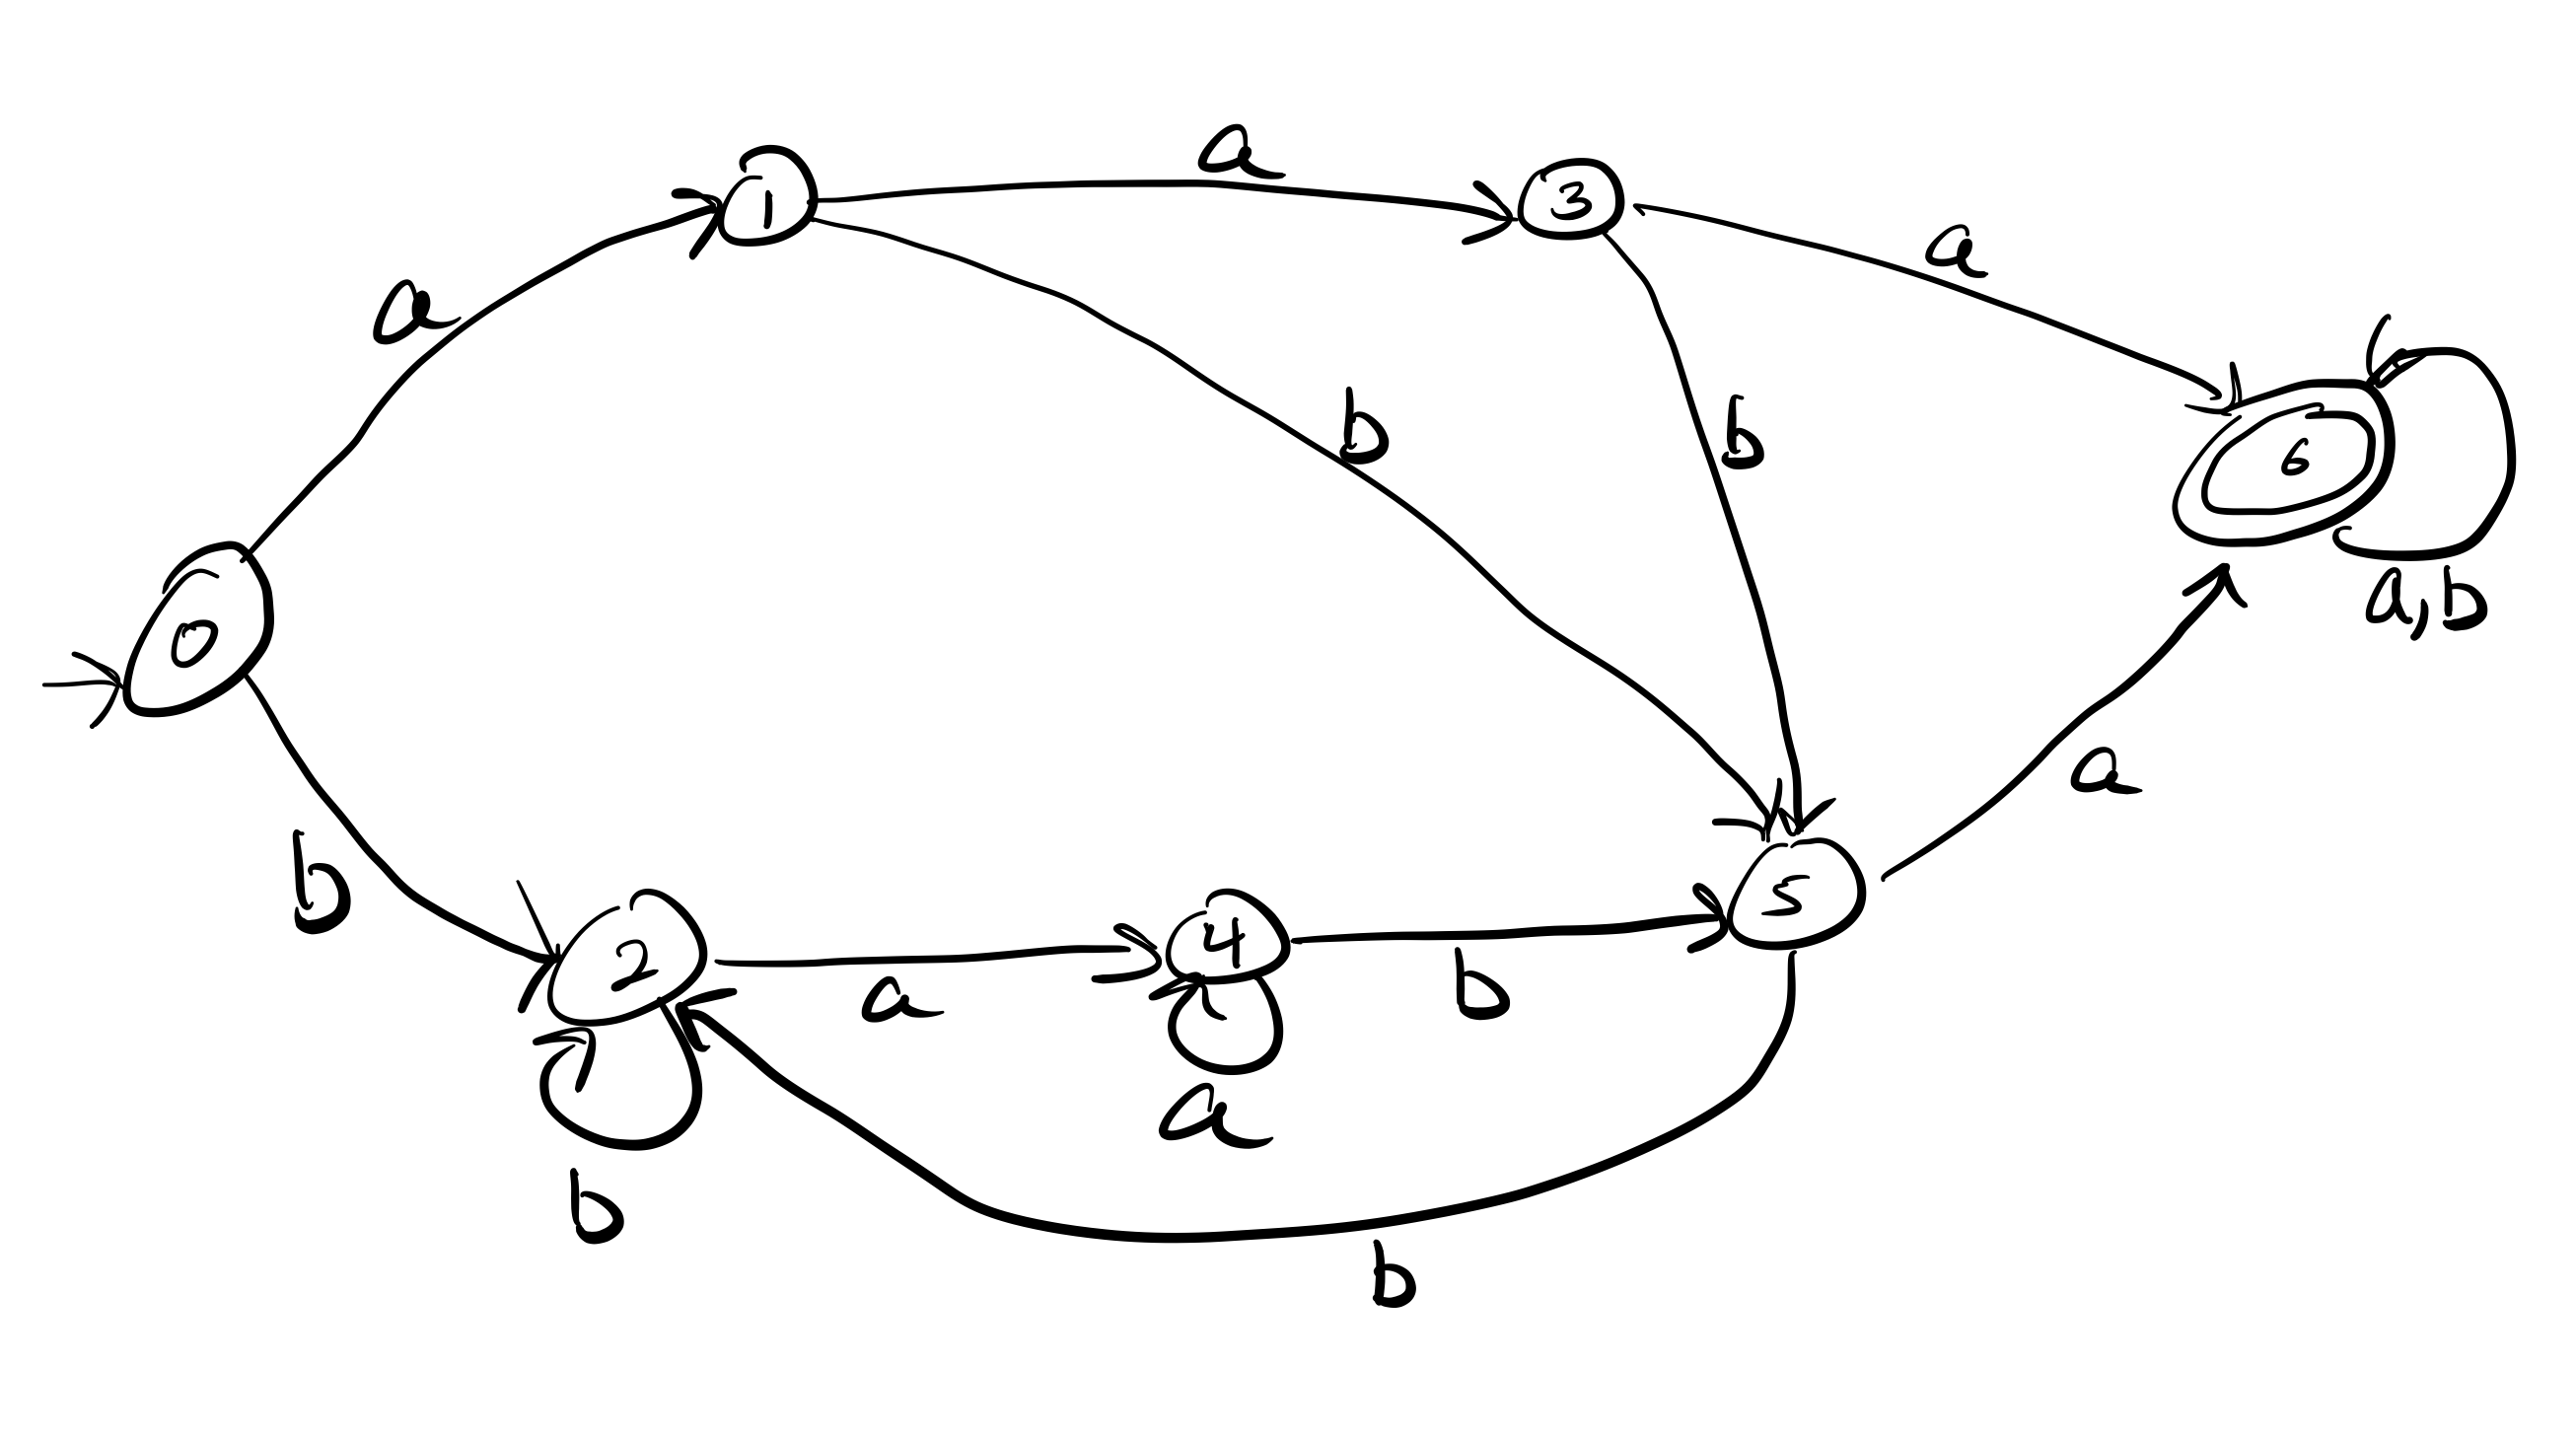
\includegraphics[scale=0.20]{problem_4.png}

This DFA consists of 7 states, $q=[7]$, where $q_0 = 0$ is the start state and 6 is the only accept state (i.e. $f=\{6\}$). The alphabet $A$ is defined as $A = \{a, b\}$. The transition function is defined as $\delta: (q_i, x \in A) \to q_i$, which is encoded into the DFA graph. Naturally, there is only one outbound arrow for each element in our alphabet.

This DFA is correct because the regular expression is broken into two subexpressions of an OR expression. The upper path (states 0, 1, 3, 6) handle the first subexpression $(aaa(a|b)^*)$ and hence return 1 on inputs matching this pattern. The following paths handle the $aba$ sub expression found in $\left((a|b)^*aba(a|b)^*\right)$: (0, 1, 5, 6), (1, 3, 5, 6), (2, 4, 5, 6). The remaining transitions are used to support the $(a|b)^*$ found in both subexpressions of the OR. If an $aaa$ or an $aba$ is not in the input string, this DFA will return 0. 

\newpage

\textbf{Problem 5 (20 points):} Given a function $f:\{0,1\}^* \to \{0,1\}$, let $f^R:\{0,1\}^* \to \{0,1\}$ be the function given by $f^R(x_1,\ldots,x_n) = 1$ if and only if $f(x_n,\ldots,x_1) = 1$.
Prove that if $f$ is computed by a DFA, then so is $f^R$. 


\textbf{Solution 5:}%  (write your solution here)

The proof is by strong induction on the length of the regular expression. We know that regular expressions are equivalent to DFAs so it will be sufficient to show that we can reverse a regular expression to detect reversed strings.

\textbf{Base cases:}
\begin{enumerate}
	\item The reverse of the single bit 0 is still 0.
	\item The reverse of the single bit 1 is still 1.
	\item The reverse of the empty string $\varepsilon$ is still $\varepsilon$.
  \end{enumerate}

\textbf{Inductive hypothesis:} Suppose all regular expressions of length $\leq k$ satisfy the following condition: if the regular expression matches the strings upon which $f$ returns 1, then we can construct a reversed regular expression that will match strings where $f^R$ returns 1. 

\textbf{Induction step:} We now show the 3 cases of adding to the length of the regular expression (i.e. k + 1).

For all the cases below, by the inductive hypothesis, each subexpression $e_i$ can be reversed since its length is less than or equal to $k$. Superscript $R$ in $e_i^R$ denotes reversal of any sub expressions.

\begin{enumerate}
	\item \textbf{Concatenation}: If $e = e_0e_1$ is a regular expression that is the concatenation of two sub expressions and $e$ matches strings where $f$ returns 1, then we can construct a new expression $e' = e_1^Re_0^R$ and $e'$ will match strings where $f^R$ returns 1.
	\item \textbf{OR}: If $e = (e_0 | e_1)$ is a regular expression that is the OR of two sub expressions and $e$ matches strings where $f$ returns 1, then we can construct a new expression $e' = (e_0^R | e_1^R)$ and $e'$ will match strings where $f^R$ returns 1.
	\item \textbf{Kleene star}: If $e = (e_0)*$ is a regular expression that uses the Kleene star and $e$ matches strings where $f$ returns 1, then we can construct a new expression $e' = (e_0^R)*$ and $e'$ will match strings where $f^R$ returns 1.
  \end{enumerate}


\textbf{Conclusion:} We can be sure of the correctness of the above cases since in each case we demonstrated that a regular expression (which is equivalent to a DFA) matches strings of the form $x_n,\ldots,x_1$ (i.e. $f(x_n,\ldots,x_1) = 1$). Our procedure creates reversed regular expressions that match reversed strings of the form $x = x_1,\ldots,x_n$ (i.e. $f^R(x_1,\ldots,x_n) = 1$), which is what we needed to show. From this we conclude that if $f$ is computed by a DFA, then so is $f^R$. 

\newpage

\textbf{Problem 6 (20 points):} Prove that the function $f:\{0,1\}^* \to \{0,1\}$ given by $f(x) = 1$ if and only if $x \in \{0^m 1 0^n 1 0^{mn} | m,n \in \N\}$ is not computed by any DFA.

\textbf{Solution 6:}% (write your solution here)

We use the pumping lemma to prove that $f:\{0,1\}^* \to \{0,1\}$ is not regular and is therefore not computed by any DFA since all regular functions can be computed by DFAs. The proof is by contradiction. We assume that $f$ is a regular function. Let $p$ be the pumping length given by the pumping lemma. Let $s$ be the string $0^p 1 0^n 1 0^{pn}$. Further let the language $A = \{0^m 1 0^n 1 0^{mn} | m,n \in \N\}$.

With $s \in A$ and having length more than $p$, the pumping lemma guarantees that s can be split into three pieces, $s = xyz$, where for any $i \geq 0$ the string $xy^iz \in A$. The pumping lemma also says that when pumping $s$, it must be divided so that $|xy| \leq p$ and $|y| > 0$. If $|xy| \leq p$, then $y$ must consist only of 0s, so $xyyz \notin A$. Therefore, $s$ cannot be pumped. Therefore, we conclude that the function $f$ is not regular and that it is not computed by any DFA.

\end{document}
